\documentclass[12pt]{article}
\usepackage[margin=1in]{geometry}
\usepackage{amsmath,amssymb,mathtools}
\usepackage{enumitem}
\usepackage{bm}
\usepackage{hyperref}
\usepackage{fancyhdr}
\usepackage{draftwatermark}
\usepackage{xcolor}
\usepackage{pgfplots}
\usepackage{titlesec}
\pgfplotsset{compat=newest}

%------------- TITLE AND METADATA -------------
\newcommand{\CourseCode}{HE2002 }
\newcommand{\CourseName}{Macroeconomics II}
\newcommand{\DocType}{Tutorial 11}

\title{
\CourseCode \CourseName \\[0.3em]
\large \DocType
}
\author{
  Academic Year 2025/2026, Semester 2 \\[0.25em]
  \textit{Quantitative Research Society @NTU}
}
\date{\today}

%------------- HEADER & FOOTER (for page 2 onward) -------------
\fancypagestyle{main}{
  \fancyhf{}
  \fancyhead[L]{\CourseCode \CourseName \ --\ \DocType}
  \fancyhead[R]{\href{https://qrsntu.org}{QRS@NTU}}
  \fancyfoot[C]{\thepage}
  \renewcommand{\headrulewidth}{0.4pt}
  \renewcommand{\footrulewidth}{0pt}
}

%------------- SIMPLE FOOTER (page 1 only) -------------
\fancypagestyle{plainfirst}{
  \fancyhf{}
  \renewcommand{\headrulewidth}{0pt}
  \renewcommand{\footrulewidth}{0pt}
  \fancyfoot[C]{\scriptsize\textcolor{gray}{\textit{For academic reference only. This document is provided for educational purposes and does not constitute an official question paper, answer key, or any formally authorised academic material. Its content is not guaranteed to be complete or accurate.}}}
}

%------------- WATERMARK -------------
\SetWatermarkText{Unofficial — QRS@NTU — qrsntu.org}
\SetWatermarkScale{1}
\SetWatermarkLightness{0.99}

%------------- SHORTCUTS -------------
\newcommand{\R}{\mathbb{R}}
\newcommand{\Rp}{\mathbb{R}_+}
\newcommand{\E}{\mathbb{E}}
\newcommand{\Var}{\mathrm{Var}}
\newcommand{\dotp}{\cdot}

%------------- STYLE -------------
\setlist[enumerate]{itemsep=0.32em, topsep=0.32em}
\setlist[itemize]{itemsep=0.22em, topsep=0.22em}

\titleformat{\subsubsection}[block]
{\normalfont\large\bfseries}
{}
{0pt}
{}

\titleformat{\paragraph}[block]
{\normalfont\normalsize\bfseries}
{}
{0pt}
{}

\titlespacing*{\paragraph}
{0pt}
{1.2ex}
{0.6ex}

\setcounter{secnumdepth}{0}
\setcounter{tocdepth}{4}

\begin{document}

\maketitle
\thispagestyle{plainfirst}
\pagestyle{main}
\bigskip

%====================================================
% OVERVIEW
%====================================================
\begin{center}
  \rule{0.8\textwidth}{0.4pt}\\[4pt]
  \textbf{Overview}\\[2pt]
  \rule{0.8\textwidth}{0.4pt}
\end{center}

\noindent
This tutorial covers:
\begin{itemize}[leftmargin=*]
  \item steady states in the Solow model with and without effective labour;
  \item per-worker and per-effective-worker transformations of production functions;
  \item steady-state output, capital, and consumption under alternative saving and depreciation rates;
  \item the consumption-maximising saving rate and its graphical interpretation;
  \item balanced-growth implications of technological progress and labour-force growth.
\end{itemize}

\bigskip

\newpage
\tableofcontents

\newpage
%====================================================
% QUESTION 1
%====================================================
\section{Question 1: Steady State and the Consumption-Maximising Saving Rate}

\noindent
Chapter 11, Q6.

\subsection{Problem}
Suppose that an economy is characterized by the following production function
\[
Y = 3\sqrt{K}\sqrt{N}.
\]

\begin{enumerate}[label=(\alph*)]
    \item Derive the steady-state level of output per worker and the steady-state level of capital per worker in terms of the saving rate, \(s\), and the depreciation rate, \(\delta\).
    \item Derive the equation for the steady-state level of consumption per worker in terms of the saving rate, \(s\), and the depreciation rate, \(\delta\).
    \item Suppose that \(\delta = 0.02\), compute the steady-state consumption per worker and steady-state output per worker when \(s = 0;\ s = 0.1;\ s = 0.2;\ s = 1\). What do you observe?
    \item Using your favorite spreadsheet software, plot your results on a graph showing the relationship between the saving rate (on the X axis) and consumption per worker (on the Y axis). Is there a saving rate that maximizes consumption per worker? Explain.
\end{enumerate}

\newpage
\subsection{Solution}

\subsubsection{Method 1: Direct steady-state algebra in per-worker form}
Let
\[
k:=\frac{K}{N},
\qquad
y:=\frac{Y}{N},
\qquad
c:=\frac{C}{N}.
\]
Starting from
\[
Y=3\sqrt{K}\sqrt{N},
\]
divide both sides by \(N\):
\[
\frac{Y}{N}=3\frac{\sqrt{K}\sqrt{N}}{N}
=3\sqrt{\frac{K}{N}}
=3\sqrt{k}.
\]
Hence the per-worker production function is
\[
y=3\sqrt{k}.
\]

With no population growth and no technological progress, the Solow law of motion for capital per worker is
\[
k_{t+1}-k_t=s y_t-\delta k_t.
\]
At the steady state,
\[
k_{t+1}=k_t=k^*,
\]
so
\[
s y^*=\delta k^*.
\]
Substituting \(y^*=3\sqrt{k^*}\),
\[
3s\sqrt{k^*}=\delta k^*.
\]

\begin{enumerate}[label=(\alph*)]
    \item
    Solve
    \[
    3s\sqrt{k^*}=\delta k^*.
    \]
    For the positive steady state, divide both sides by \(\sqrt{k^*}\):
    \[
    3s=\delta \sqrt{k^*}.
    \]
    Hence
    \[
    \sqrt{k^*}=\frac{3s}{\delta},
    \qquad
    k^*=\left(\frac{3s}{\delta}\right)^2.
    \]
    Therefore the steady-state capital per worker is
    \[
    \boxed{k^*=\left(\frac{3s}{\delta}\right)^2.}
    \]

    The steady-state output per worker is
    \[
    y^*=3\sqrt{k^*}
    =3\left(\frac{3s}{\delta}\right)
    =\frac{9s}{\delta}.
    \]
    Therefore
    \[
    \boxed{y^*=\frac{9s}{\delta}.}
    \]

    \item
    Steady-state consumption per worker is
    \[
    c^*=(1-s)y^*.
    \]
    Using part (a),
    \[
    c^*=(1-s)\frac{9s}{\delta}.
    \]
    Expanding,
    \[
    c^*=\frac{9}{\delta}(s-s^2).
    \]
    Thus
    \[
    \boxed{c^*=\frac{9s(1-s)}{\delta}=\frac{9}{\delta}(s-s^2).}
    \]

    \item
    Now set \(\delta=0.02\). Then
    \[
    y^*=\frac{9s}{0.02}=450s,
    \qquad
    c^*=\frac{9s(1-s)}{0.02}=450s(1-s).
    \]

    \paragraph{Case \(s=0\).}
    \[
    y^*=450(0)=0,
    \qquad
    c^*=450(0)(1-0)=0.
    \]

    \paragraph{Case \(s=0.1\).}
    \[
    y^*=450(0.1)=45,
    \qquad
    c^*=450(0.1)(0.9)=40.5.
    \]

    \paragraph{Case \(s=0.2\).}
    \[
    y^*=450(0.2)=90,
    \qquad
    c^*=450(0.2)(0.8)=72.
    \]

    \paragraph{Case \(s=1\).}
    \[
    y^*=450(1)=450,
    \qquad
    c^*=450(1)(0)=0.
    \]

    Therefore,
    \[
    \boxed{
    \begin{array}{c|cccc}
    s & 0 & 0.1 & 0.2 & 1 \\ \hline
    y^* & 0 & 45 & 90 & 450 \\
    c^* & 0 & 40.5 & 72 & 0
    \end{array}}
    \]

    We observe that steady-state output per worker rises with the saving rate, but steady-state consumption per worker does not. Consumption is zero when \(s=0\) and also zero when \(s=1\), so it must rise at first and then fall.

    \item
    Since
    \[
    c^*=\frac{9}{\delta}(s-s^2),
    \]
    the graph of steady-state consumption per worker against \(s\) is a downward-opening parabola.

    To find the maximizing saving rate, differentiate:
    \[
    \frac{dc^*}{ds}
    =\frac{9}{\delta}(1-2s).
    \]
    Set this equal to zero:
    \[
    1-2s=0
    \quad\Longrightarrow\quad
    s=\frac12.
    \]
    The second derivative is
    \[
    \frac{d^2c^*}{ds^2}=-\frac{18}{\delta}<0,
    \]
    so this indeed gives a maximum.

    Thus the saving rate that maximizes steady-state consumption per worker is
    \[
    \boxed{s^{GR}=\frac12.}
    \]

    When \(\delta=0.02\), the maximum steady-state consumption per worker is
    \[
    c^*_{\max}
    =\frac{9}{0.02}\left(\frac12-\frac14\right)
    =450\cdot \frac14
    =112.5.
    \]
    Hence
    \[
    \boxed{c^*_{\max}=112.5 \text{ when } \delta=0.02.}
    \]

    A suitable graph is:

    \begin{center}
    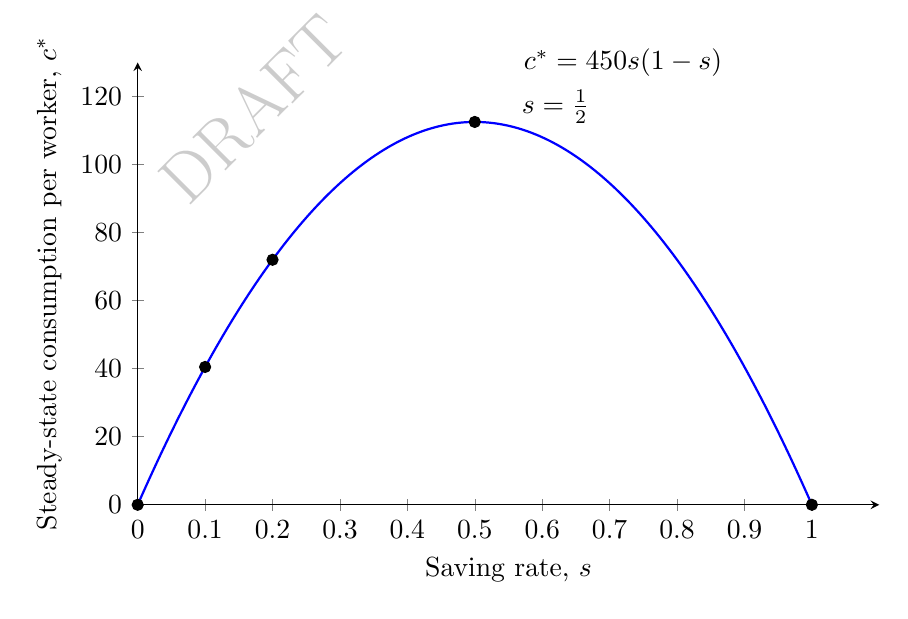
\begin{tikzpicture}
    \begin{axis}[
        width=11cm,
        height=7.2cm,
        xmin=0,xmax=1.1,
        ymin=0,ymax=130,
        axis lines=left,
        xlabel={Saving rate, \(s\)},
        ylabel={Steady-state consumption per worker, \(c^*\)},
        xtick={0,0.1,0.2,0.3,0.4,0.5,0.6,0.7,0.8,0.9,1},
        ytick={0,20,40,60,80,100,120},
        clip=false
    ]
    \addplot[domain=0:1,samples=200,thick,blue] {450*x*(1-x)};
    \addplot[only marks,mark=*,mark size=2pt] coordinates {(0,0) (0.1,40.5) (0.2,72) (0.5,112.5) (1,0)};
    \node at (axis cs:0.72,130) {\(c^*=450s(1-s)\)};
    \node at (axis cs:0.62,117) {\(s=\frac12\)};
    \end{axis}
    \end{tikzpicture}
    \end{center}

    Therefore,
    \begin{center}
    \fbox{\parbox{0.9\linewidth}{\centering
    Yes. The saving rate that maximizes steady-state consumption per worker is $s=\frac12$.
    }}
    \end{center}
\end{enumerate}

\subsubsection{Method 2: Golden-rule interpretation and break-even investment}
Again, the per-worker production function is
\[
y=f(k)=3\sqrt{k}.
\]
In steady state,
\[
sf(k)=\delta k.
\]
Steady-state consumption per worker can also be written as
\[
c^*=y^*-\delta k^*,
\]
because at the steady state investment per worker equals depreciation per worker.

\begin{enumerate}[label=(\alph*)]
    \item
    Use
    \[
    s f(k^*)=\delta k^*,
    \qquad
    f(k)=3\sqrt{k}.
    \]
    Then
    \[
    3s\sqrt{k^*}=\delta k^*.
    \]
    As before,
    \[
    \sqrt{k^*}=\frac{3s}{\delta},
    \qquad
    k^*=\left(\frac{3s}{\delta}\right)^2.
    \]
    Hence
    \[
    y^*=3\sqrt{k^*}=3\cdot \frac{3s}{\delta}=\frac{9s}{\delta}.
    \]
    Therefore
    \[
    \boxed{k^*=\left(\frac{3s}{\delta}\right)^2,\qquad y^*=\frac{9s}{\delta}.}
    \]

    \item
    Using
    \[
    c^*=f(k^*)-\delta k^*,
    \]
    we obtain
    \[
    c^*=3\sqrt{k^*}-\delta k^*.
    \]
    Substituting
    \[
    \sqrt{k^*}=\frac{3s}{\delta},
    \qquad
    k^*=\left(\frac{3s}{\delta}\right)^2,
    \]
    gives
    \[
    c^*=3\left(\frac{3s}{\delta}\right)-\delta \left(\frac{3s}{\delta}\right)^2
    =\frac{9s}{\delta}-\frac{9s^2}{\delta}
    =\frac{9s(1-s)}{\delta}.
    \]
    Hence
    \[
    \boxed{c^*=\frac{9s(1-s)}{\delta}.}
    \]

    \item
    With \(\delta=0.02\),
    \[
    k^*=\left(\frac{3s}{0.02}\right)^2=(150s)^2=22500s^2,
    \qquad
    y^*=450s,
    \qquad
    c^*=450s(1-s).
    \]
    Therefore:
    \[
    \boxed{
    \begin{array}{c|cccc}
    s & 0 & 0.1 & 0.2 & 1 \\ \hline
    k^* & 0 & 225 & 900 & 22500 \\
    y^* & 0 & 45 & 90 & 450 \\
    c^* & 0 & 40.5 & 72 & 0
    \end{array}}
    \]

    The notable pattern is that higher saving always raises \(k^*\) and \(y^*\), but not necessarily \(c^*\). Very high saving can lower consumption because too much output is diverted into investment.

    \item
    A conceptually distinct way to find the consumption-maximizing saving rate is to maximize steady-state consumption with respect to \(k\), not directly with respect to \(s\). In the steady state,
    \[
    c^*=f(k)-\delta k = 3\sqrt{k}-\delta k.
    \]
    Differentiate with respect to \(k\):
    \[
    \frac{dc^*}{dk}=\frac{3}{2\sqrt{k}}-\delta.
    \]
    Set equal to zero:
    \[
    \frac{3}{2\sqrt{k}}=\delta
    \quad\Longrightarrow\quad
    \sqrt{k}=\frac{3}{2\delta}.
    \]
    Thus the golden-rule capital stock is
    \[
    k^{GR}=\left(\frac{3}{2\delta}\right)^2.
    \]
    At a steady state, the saving rate that supports a given \(k\) satisfies
    \[
    s=\frac{\delta k}{f(k)}
    =\frac{\delta k}{3\sqrt{k}}
    =\frac{\delta \sqrt{k}}{3}.
    \]
    Substituting \(\sqrt{k^{GR}}=\frac{3}{2\delta}\),
    \[
    s^{GR}=\frac{\delta}{3}\cdot \frac{3}{2\delta}=\frac12.
    \]
    Hence
    \[
    \boxed{s^{GR}=\frac12.}
    \]

    So there is indeed a unique saving rate that maximizes steady-state consumption per worker. It is the rate that supports the golden-rule capital stock.
\end{enumerate}

\newpage
%====================================================
% QUESTION 2
%====================================================
\section{Question 2: Steady State with Technological Progress and Population Growth}

\noindent
Chapter 12, Q6

\subsection{Problem}
Suppose that the economy’s production function is
\[
Y = K^{1/2}(AN)^{1/2},
\]
that the saving rate, \(s\), is equal to 16\%, and that the rate of depreciation, \(\delta\), is equal to 10\%. Suppose further that the number of workers grows at 2\% per year and that the rate of technological progress is 4\% per year.

To solve for the steady-state values of capital stock per effective worker \(\left(\frac{K}{AN}\right)^*\) and output per effective worker \(\left(\frac{Y}{AN}\right)^*\), we use the condition that actual investment \(I\) equals required investment \(I_R\). This allows us to determine the steady-state level of capital per effective worker \(\left(\frac{K}{AN}\right)^*\).

In our model with technological progress:
\[
I = sY,\qquad I_R = (\delta + g_A + g_N)K
\]
\[
I = I_R \Rightarrow sY = (\delta + g_A + g_N)K \Rightarrow s\frac{Y}{AN} = (\delta + g_A + g_N)\frac{K}{AN} \Rightarrow s f\!\left(\frac{K}{AN}\right) = (\delta + g_A + g_N)\frac{K}{AN}
\]

The value of capital per effective worker that satisfies the equation above is the steady-state level of capital stock per effective worker, denoted as \(\left(\frac{K}{AN}\right)^*\).

\begin{enumerate}[label=(\alph*)]
    \item Find the steady-state values of the variables listed in (1) through (5).
    \begin{enumerate}[label=\roman*.]
        \item The capital stock per effective worker.
        \item Output per effective worker.
        \item The growth rate of output per effective worker.
        \item The growth rate of output per worker.
        \item The growth rate of output.
    \end{enumerate}

    \item Suppose that the rate of technological progress doubles to 8\% per year. Recompute the answers to part a.
    \begin{enumerate}[label=\roman*.]
        \item The capital stock per effective worker.
        \item Output per effective worker.
        \item The growth rate of output per effective worker.
        \item The growth rate of output per worker.
        \item The growth rate of output.
    \end{enumerate}

    \item Now suppose that the rate of technological progress is still equal to 4\%, but the number of workers now grows at 6\% per year. Recompute the answers to part a. Are people better off in part a or part c? Explain.
    \begin{enumerate}[label=\roman*.]
        \item The capital stock per effective worker.
        \item Output per effective worker.
        \item The growth rate of output per effective worker.
        \item The growth rate of output per worker.
        \item The growth rate of output.
    \end{enumerate}
\end{enumerate}

\newpage
\subsection{Solution}

\subsubsection{Method 1: Direct effective-worker steady-state algebra}
Define capital per effective worker and output per effective worker by
\[
\tilde{k}:=\frac{K}{AN},
\qquad
\tilde{y}:=\frac{Y}{AN}.
\]
Given
\[
Y=K^{1/2}(AN)^{1/2},
\]
divide by \(AN\):
\[
\tilde{y}
=
\frac{K^{1/2}(AN)^{1/2}}{AN}
=
\left(\frac{K}{AN}\right)^{1/2}
=
\tilde{k}^{1/2}.
\]
So the per-effective-worker production function is
\[
\tilde{y}=f(\tilde{k})=\sqrt{\tilde{k}}.
\]

In steady state with technological progress and labour-force growth,
\[
s f(\tilde{k}^*)=(\delta+g_A+g_N)\tilde{k}^*.
\]
With \(f(\tilde{k})=\sqrt{\tilde{k}}\), this becomes
\[
s\sqrt{\tilde{k}^*}=(\delta+g_A+g_N)\tilde{k}^*.
\]
For the positive steady state,
\[
\sqrt{\tilde{k}^*}=\frac{s}{\delta+g_A+g_N},
\qquad
\tilde{k}^*=\left(\frac{s}{\delta+g_A+g_N}\right)^2,
\]
and
\[
\tilde{y}^*=\sqrt{\tilde{k}^*}=\frac{s}{\delta+g_A+g_N}.
\]

\begin{enumerate}[label=(\alph*)]
    \item
    Here
    \[
    s=0.16,\qquad \delta=0.10,\qquad g_A=0.04,\qquad g_N=0.02.
    \]
    Therefore
    \[
    \delta+g_A+g_N=0.10+0.04+0.02=0.16.
    \]
    So
    \[
    \tilde{k}^*=\left(\frac{0.16}{0.16}\right)^2=1,
    \qquad
    \tilde{y}^*=\frac{0.16}{0.16}=1.
    \]

    In steady state, output per effective worker is constant, so its growth rate is
    \[
    g_{\tilde{y}}=0.
    \]
    Output per worker is
    \[
    \frac{Y}{N}=A\cdot \frac{Y}{AN}=A\tilde{y},
    \]
    so in steady state its growth rate is
    \[
    g_{Y/N}=g_A+g_{\tilde{y}}=g_A=4\%.
    \]
    Total output is
    \[
    Y=(AN)\tilde{y},
    \]
    so its growth rate is
    \[
    g_Y=g_A+g_N+g_{\tilde{y}}=g_A+g_N=6\%.
    \]

    Therefore,
    \[
    \boxed{
    \begin{aligned}
    \text{i. } & \left(\frac{K}{AN}\right)^*=1,\\
    \text{ii. } & \left(\frac{Y}{AN}\right)^*=1,\\
    \text{iii. } & g_{Y/(AN)}=0,\\
    \text{iv. } & g_{Y/N}=4\%,\\
    \text{v. } & g_Y=6\%.
    \end{aligned}}
    \]

    \item
    Now let technological progress double to \(8\%\), so
    \[
    g_A=0.08.
    \]
    Then
    \[
    \delta+g_A+g_N=0.10+0.08+0.02=0.20.
    \]
    Hence
    \[
    \tilde{k}^*=\left(\frac{0.16}{0.20}\right)^2=(0.8)^2=0.64,
    \qquad
    \tilde{y}^*=\frac{0.16}{0.20}=0.8.
    \]
    Again, in steady state,
    \[
    g_{Y/(AN)}=0.
    \]
    Output per worker grows at
    \[
    g_{Y/N}=g_A=8\%.
    \]
    Output grows at
    \[
    g_Y=g_A+g_N=8\%+2\%=10\%.
    \]

    Therefore,
    \[
    \boxed{
    \begin{aligned}
    \text{i. } & \left(\frac{K}{AN}\right)^*=0.64,\\
    \text{ii. } & \left(\frac{Y}{AN}\right)^*=0.8,\\
    \text{iii. } & g_{Y/(AN)}=0,\\
    \text{iv. } & g_{Y/N}=8\%,\\
    \text{v. } & g_Y=10\%.
    \end{aligned}}
    \]

    \item
    Now return to \(g_A=0.04\), but let the growth rate of workers rise to
    \[
    g_N=0.06.
    \]
    Then
    \[
    \delta+g_A+g_N=0.10+0.04+0.06=0.20.
    \]
    Therefore
    \[
    \tilde{k}^*=\left(\frac{0.16}{0.20}\right)^2=0.64,
    \qquad
    \tilde{y}^*=\frac{0.16}{0.20}=0.8.
    \]
    In steady state,
    \[
    g_{Y/(AN)}=0.
    \]
    Output per worker grows at
    \[
    g_{Y/N}=g_A=4\%.
    \]
    Output grows at
    \[
    g_Y=g_A+g_N=4\%+6\%=10\%.
    \]

    Hence
    \[
    \boxed{
    \begin{aligned}
    \text{i. } & \left(\frac{K}{AN}\right)^*=0.64,\\
    \text{ii. } & \left(\frac{Y}{AN}\right)^*=0.8,\\
    \text{iii. } & g_{Y/(AN)}=0,\\
    \text{iv. } & g_{Y/N}=4\%,\\
    \text{v. } & g_Y=10\%.
    \end{aligned}}
    \]

    People are better off in part a than in part c, because the steady-state level of output per effective worker is higher in part a:
    \[
    1 > 0.8.
    \]
    Also, since \(g_A\) is the same in parts a and c, the growth rate of output per worker is the same, namely \(4\%\), but the level of output per worker is lower in part c because \(\tilde{y}^*\) is lower.

    Therefore,
    \[
    \boxed{\text{People are better off in part a than in part c.}}
    \]
\end{enumerate}

\newpage
\subsubsection{Method 2: Balanced-growth-path interpretation}
A conceptually different way to proceed is to start from the balanced-growth properties of the Solow model with effective labour.

From
\[
Y=K^{1/2}(AN)^{1/2},
\]
if we divide by \(AN\), we obtain
\[
\frac{Y}{AN}=\left(\frac{K}{AN}\right)^{1/2}.
\]
Thus constant \(\frac{K}{AN}\) implies constant \(\frac{Y}{AN}\). So on the balanced-growth path:
\begin{itemize}[leftmargin=*]
    \item capital per effective worker is constant;
    \item output per effective worker is constant;
    \item output per worker grows at the rate of technological progress \(g_A\);
    \item total output grows at the rate \(g_A+g_N\).
\end{itemize}

To pin down the constant level of \(\tilde{k}\), use the steady-state investment condition:
\[
s\tilde{y}=(\delta+g_A+g_N)\tilde{k}.
\]
Since \(\tilde{y}=\sqrt{\tilde{k}}\), this gives
\[
s\sqrt{\tilde{k}}=(\delta+g_A+g_N)\tilde{k},
\]
hence
\[
\sqrt{\tilde{k}^*}=\frac{s}{\delta+g_A+g_N},
\qquad
\tilde{k}^*=\left(\frac{s}{\delta+g_A+g_N}\right)^2,
\qquad
\tilde{y}^*=\frac{s}{\delta+g_A+g_N}.
\]

\begin{enumerate}[label=(\alph*)]
    \item
    Since
    \[
    \delta+g_A+g_N=0.10+0.04+0.02=0.16,
    \]
    we get
    \[
    \tilde{k}^*=1,
    \qquad
    \tilde{y}^*=1.
    \]
    Balanced-growth implications then give
    \[
    g_{Y/(AN)}=0,
    \qquad
    g_{Y/N}=g_A=4\%,
    \qquad
    g_Y=g_A+g_N=6\%.
    \]
    Therefore,
    \[
    \boxed{
    \begin{aligned}
    \left(\frac{K}{AN}\right)^*&=1,\\
    \left(\frac{Y}{AN}\right)^*&=1,\\
    g_{Y/(AN)}&=0,\\
    g_{Y/N}&=4\%,\\
    g_Y&=6\%.
    \end{aligned}}
    \]

    \item
    If \(g_A\) doubles to \(8\%\), then
    \[
    \delta+g_A+g_N=0.10+0.08+0.02=0.20.
    \]
    So
    \[
    \tilde{k}^*=\left(\frac{0.16}{0.20}\right)^2=0.64,
    \qquad
    \tilde{y}^*=\frac{0.16}{0.20}=0.8.
    \]
    Since effective-worker variables are constant on the balanced-growth path,
    \[
    g_{Y/(AN)}=0.
    \]
    Meanwhile,
    \[
    g_{Y/N}=g_A=8\%,
    \qquad
    g_Y=g_A+g_N=10\%.
    \]
    Hence
    \[
    \boxed{
    \begin{aligned}
    \left(\frac{K}{AN}\right)^*&=0.64,\\
    \left(\frac{Y}{AN}\right)^*&=0.8,\\
    g_{Y/(AN)}&=0,\\
    g_{Y/N}&=8\%,\\
    g_Y&=10\%.
    \end{aligned}}
    \]

    \item
    If \(g_A=4\%\) and \(g_N=6\%\), then once again
    \[
    \delta+g_A+g_N=0.10+0.04+0.06=0.20.
    \]
    So the steady-state effective-worker levels are the same as in part b:
    \[
    \tilde{k}^*=0.64,
    \qquad
    \tilde{y}^*=0.8.
    \]
    But the growth decomposition changes:
    \[
    g_{Y/(AN)}=0,
    \qquad
    g_{Y/N}=g_A=4\%,
    \qquad
    g_Y=g_A+g_N=10\%.
    \]
    Therefore,
    \[
    \boxed{
    \begin{aligned}
    \left(\frac{K}{AN}\right)^*&=0.64,\\
    \left(\frac{Y}{AN}\right)^*&=0.8,\\
    g_{Y/(AN)}&=0,\\
    g_{Y/N}&=4\%,\\
    g_Y&=10\%.
    \end{aligned}}
    \]

    Comparing parts a and c:
    \begin{itemize}[leftmargin=*]
        \item \(\tilde{y}^*\) is higher in part a \((1)\) than in part c \((0.8)\);
        \item output per worker grows at the same rate in both parts, because \(g_A\) is unchanged at \(4\%\);
        \item therefore the relevant welfare comparison is about the level of output per worker, which is higher in part a.
    \end{itemize}
    Thus
    \[
    \boxed{\text{Part a is better than part c because the steady-state level of output per worker is higher.}}
    \]
\end{enumerate}

\begin{center}
\renewcommand{\arraystretch}{1.25}
\begin{tabular}{|c|c|c|c|c|c|}
\hline
Case & \(\left(\frac{K}{AN}\right)^*\) & \(\left(\frac{Y}{AN}\right)^*\) & \(g_{Y/(AN)}\) & \(g_{Y/N}\) & \(g_Y\) \\
\hline
(a) \(g_A=4\%,\ g_N=2\%\) & \(1\) & \(1\) & \(0\) & \(4\%\) & \(6\%\) \\
(b) \(g_A=8\%,\ g_N=2\%\) & \(0.64\) & \(0.8\) & \(0\) & \(8\%\) & \(10\%\) \\
(c) \(g_A=4\%,\ g_N=6\%\) & \(0.64\) & \(0.8\) & \(0\) & \(4\%\) & \(10\%\) \\
\hline
\end{tabular}
\end{center}

\end{document}
